\documentclass[aspectratio=169]{beamer}
\mode<presentation>
% \usetheme{Warsaw}
% \usetheme{Goettingen}
\usetheme{Hannover}
% \useoutertheme{default}

% \useoutertheme{infolines}
\useoutertheme{sidebar}
\usecolortheme{dolphin}

\usepackage{amsmath}
\usepackage{amssymb}
\usepackage{enumerate}

% some bold math symbosl
\newcommand{\Cov}{\mathrm{Cov}}
\newcommand{\Cor}{\mathrm{Cor}}
\newcommand{\Var}{\mathrm{Var}}
\newcommand{\brho}{\boldsymbol{\rho}}
\newcommand{\bSigma}{\boldsymbol{\Sigma}}
\newcommand{\btheta}{\boldsymbol{\theta}}
\newcommand{\bbeta}{\boldsymbol{\beta}}
\newcommand{\bmu}{\boldsymbol{\mu}}
\newcommand{\bW}{\mathbf{W}}
\newcommand{\one}{\mathbf{1}}
\newcommand{\bH}{\mathbf{H}}
\newcommand{\by}{\mathbf{y}}
\newcommand{\bolde}{\mathbf{e}}
\newcommand{\bx}{\mathbf{x}}

\newcommand{\cpp}[1]{\texttt{#1}}

\title{Mathematical Biostatistics Bootcamp: Lecture 6, Likelihood}
\author{Brian Caffo}
\date{\today}
\institute[Department of Biostatistics]{
  Department of Biostatistics \\
  Johns Hopkins Bloomberg School of Public Health\\
  Johns Hopkins University
}


\begin{document}

\frame{\titlepage}


\section{Table of contents}
\frame{
  \frametitle{Table of contents}
  \tableofcontents
}


\section{Defining likelihood}
\begin{frame}\frametitle{Likelihood}
\begin{itemize}
\item A common and fruitful approach to statistics is to assume that
  the data arises from a family of distributions indexed by a
  parameter that represents a useful summary of the distribution
\item The {\bf likelihood} of a collection of data is the joint
  density evaluated as a function of the parameters with the data fixed
\item Likelihood analysis of data uses the likelihood to perform inference
  regarding the unknown parameter
\end{itemize}
\end{frame}

\begin{frame}\frametitle{Likelihood}
  Given a statistical probability mass function or density, say $f(x,
  \theta)$, where $\theta$ is an unknown parameter, the {\bf likelihood}
  is $f$ viewed as a function of $\theta$ for a fixed, observed value of
  $x$. 
\end{frame}

\section{Interpreting likelihoods}
\begin{frame}\frametitle{Interpretations of likelihoods}
The likelihood has the following properties:
  \begin{enumerate}
  \item Ratios of likelihood values measure the relative {\bf
      evidence} of one value of the unknown parameter to another.
  \item Given a statistical model and observed data, all of the relevant
    information contained in the data regarding the unknown parameter is
    contained in the likelihood.
  \item If $\{X_i\}$ are independent random variables, then their likelihoods
    multiply.  That is, the likelihood of the parameters given all of
    the $X_i$ is simply the product of the individual likelihoods.
  \end{enumerate}
\end{frame}

\begin{frame}\frametitle{Example}
\begin{itemize}
\item Suppose that we flip a coin with success probability $\theta$
\item Recall that the mass function for $x$
  $$
  f(x,\theta) = \theta^x(1 - \theta)^{1 - x}  ~~~\mbox{for}~~~ \theta \in [0,1].
  $$
  where $x$ is either $0$ (Tails) or $1$ (Heads) 
\item Suppose that the result is a head
\item The likelihood is
  $$
  {\cal L}(\theta, 1) = \theta^1 (1 - \theta)^{1 - 1} = \theta  ~~~\mbox{for} ~~~ \theta \in [0,1].
  $$
\item Therefore, ${\cal L}(.5, 1) / {\cal L}(.25, 1) = 2$, 
\item There is twice as much evidence supporting the hypothesis that $\theta = .5$ to the
hypothesis that $\theta = .25$
\end{itemize}
\end{frame}

\begin{frame}\frametitle{Example continued}
\begin{itemize}
\item   Suppose now that we flip our coin from the previous example 4 times and
  get the sequence 1, 0, 1, 1
\item The likelihood is:
  \begin{eqnarray*}
  {\cal L}(\theta, 1,0,1,1) & = & \theta^1 (1 - \theta)^{1 - 1}
  \theta^0 (1 - \theta)^{1 - 0}  \\
& \times & \theta^1 (1 - \theta)^{1 - 1} 
   \theta^1 (1 - \theta)^{1 - 1}\\
& = &  \theta^3(1 - \theta)^1
  \end{eqnarray*}
\item This likelihood only depends on the total number of heads and
  the total number of tails; we might write ${\cal L}(\theta, 1, 3)$
  for shorthand
\item Now consider ${\cal L}(.5, 1, 3) / {\cal L}(.25, 1, 3) = 5.33$
\item There is over five times as much evidence supporting the
  hypothesis that $\theta = .5$ over that $\theta = .25$
\end{itemize}
\end{frame}

\section{Plotting likelihoods}
\begin{frame}\frametitle{Plotting likelihoods}
\begin{itemize}
\item Generally, we want to consider all the values of $\theta$ between 0 and 1
\item A {\bf likelihood plot} displays $\theta$ by ${\cal
    L}(\theta,x)$
\item Usually, it is divided by its maximum value so that its height
  is 1
\item Because the likelihood measures {\em relative evidence}, dividing the
  curve by its maximum value (or any other value for that matter) does
  not change its interpretation
\end{itemize}
\end{frame}

\begin{frame}
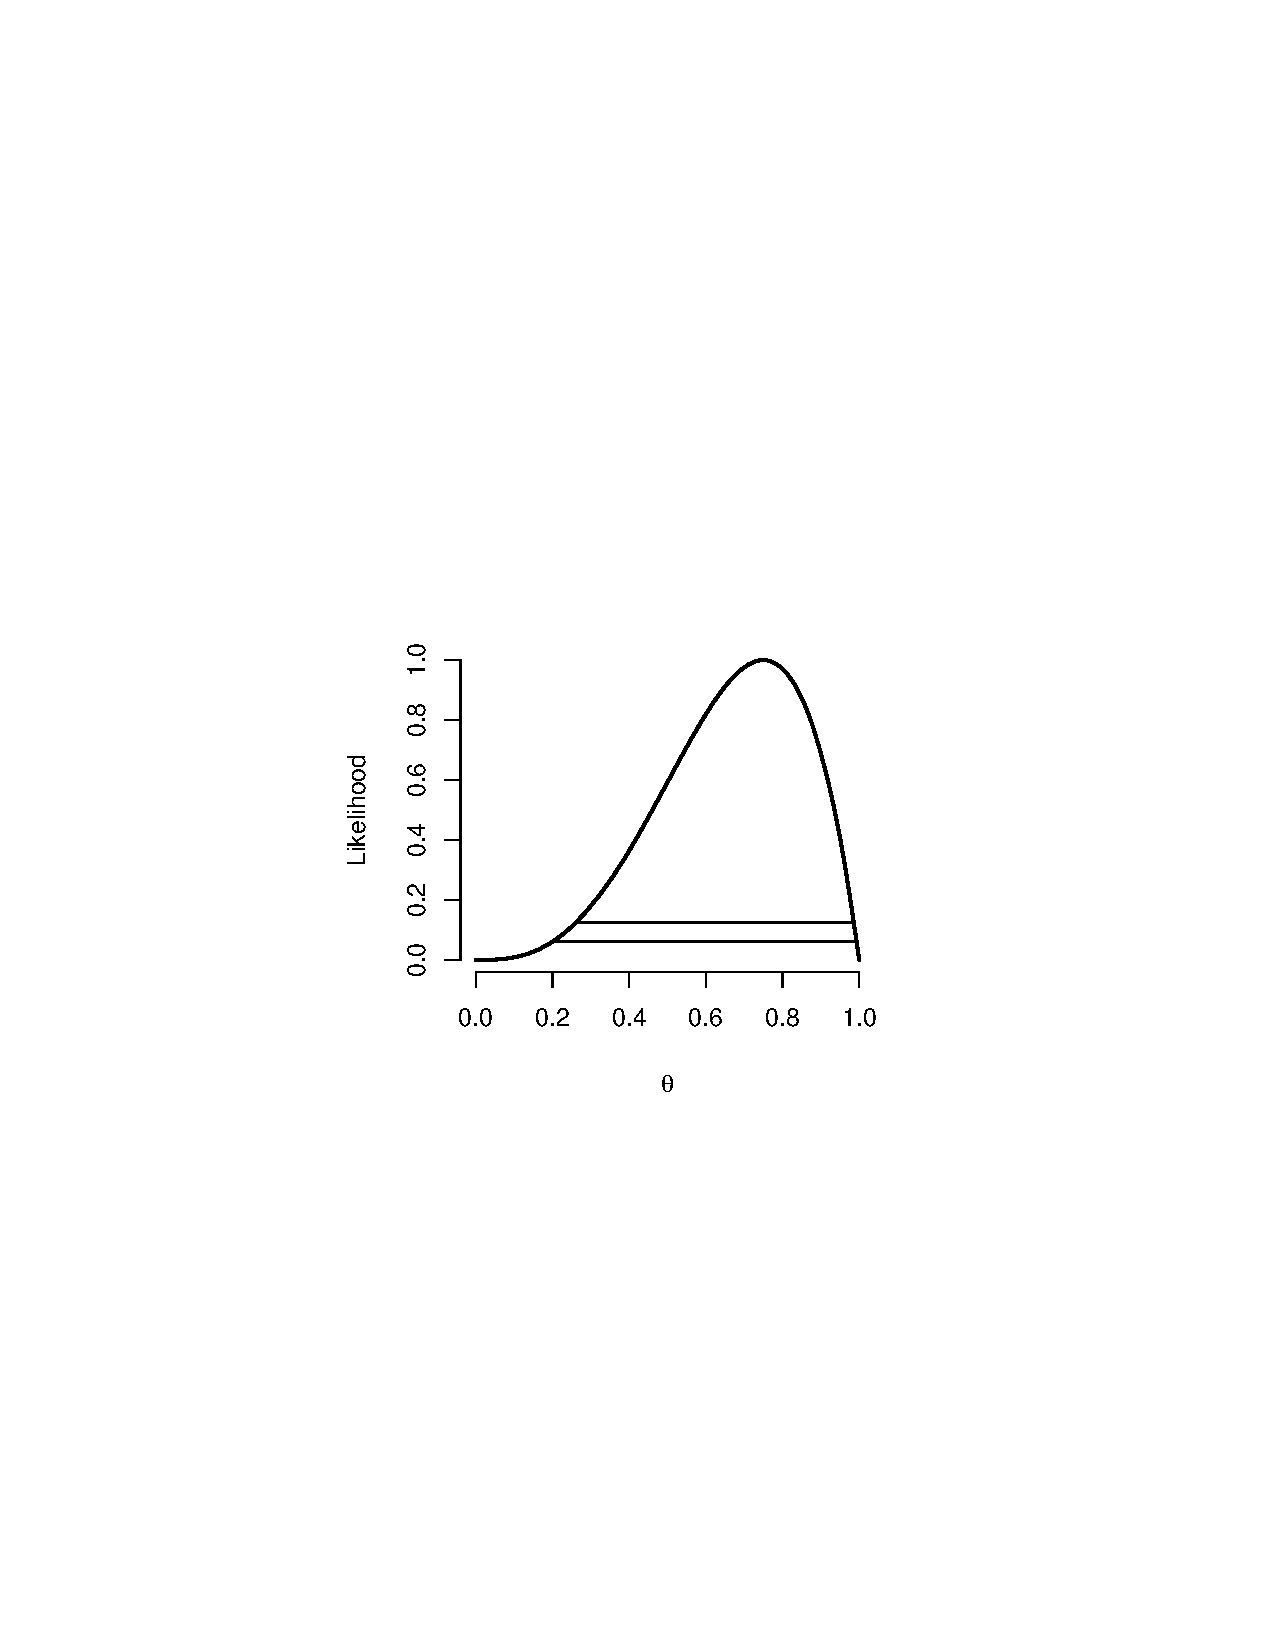
\includegraphics[width=4.5in]{coinLikelihood.pdf}
\end{frame}

\section{Maximum likelihood}
\begin{frame}\frametitle{Maximum likelihood}
\begin{itemize}
\item The value of $\theta$ where the curve reaches its maximum has a special meaning
\item It is the value of $\theta$ that is most well supported by the
  data
\item This point is called the {\bf maximum likelihood estimate} (or
  MLE) of $\theta$
  $$
  MLE = \mathrm{argmax}_\theta {\cal L}(\theta, x).
  $$
\item Another interpretation of the MLE is that it is the value of
  $\theta$ that would make the data that we observed most probable
\end{itemize}
\end{frame}

\begin{frame}\frametitle{Maximum likelihood, coin example}
\begin{itemize}
\item The maximum likelihood estimate for $\theta$ is always the proportion of heads
\item Proof: Let $x$ be the number of heads and $n$ be the number of trials
\item Recall 
$$
{\cal L}(\theta, x) = \theta^x(1-\theta)^{n-x}
$$
\item It's easier to maximize the {\bf log-likelihood}
$$
l(\theta, x) = x \log(\theta) + (n - x)\log(1 - \theta)
$$
\end{itemize}
\end{frame}

\begin{frame}\frametitle{Continued}
\begin{itemize}
\item Taking the derivative we get
$$
\frac{d}{d\theta} l(\theta, x) = \frac{x}{\theta} - \frac{n-x}{1 - \theta}
$$
\item Setting equal to zero implies
$$
(1 - \frac{x}{n})\theta = (1 - \theta) \frac{x}{n}
$$
\item Which is clearly solved at $\theta = \frac{x}{n}$
\item Notice that the second derivative
$$
\frac{d^2}{d\theta^2} l(\theta, x) = -\frac{x}{\theta^2} - \frac{n-x}{(1 - \theta)^2} < 0
$$
provided that $x$ is not $0$ or $n$ (do these cases on your own)
\end{itemize}
\end{frame}

\section{Interpreting likelihood ratios}
\begin{frame}\frametitle{What constitutes strong evidence?}
\begin{itemize}
\item Again imagine an experiment where a person repeatedly flips a
  coin
\item Consider the possibility that we are entertaining three
  hypotheses: $H_1:\theta = 0$, $H_2:\theta=.5$, and $H_3:\theta = 1$
\end{itemize}
\end{frame}

\begin{frame}
\tiny
  \begin{tabular}{rccccc}
    Outcome $X$ & $P(X ~|~ H_1)$ & $P(X ~|~ H_2)$ & $P(X ~|~ H_3)$ & ${\cal L}(H_1) / {\cal L}(H_2)$ & ${\cal L}(H_3) / {\cal L}(H_2)$ \\ \hline
H   & 0 & .5   & 1 & 0 & 2 \\
T   & 1 & .5   & 0 & 2 & 0 \\ \hline
HH  & 0 & .25  & 1 & 0 & 4 \\
HT  & 0 & .25  & 0 & 0 & 0 \\
TH  & 0 & .25  & 0 & 0 & 0 \\
TT  & 1 & .25  & 0 & 4 & 0 \\ \hline
HHH & 0 & .125 & 1 & 0 & 8 \\
HHT & 0 & .125 & 0 & 0 & 0 \\
HTH & 0 & .125 & 0 & 0 & 0 \\
THH & 0 & .125 & 0 & 0 & 0 \\
HTT & 0 & .125 & 0 & 0 & 0 \\
THT & 0 & .125 & 0 & 0 & 0 \\
TTH & 0 & .125 & 0 & 0 & 0 \\
TTT & 1 & .125 & 0 & 8 & 0 \\ \hline
  \end{tabular}
\normalsize
\end{frame}

\begin{frame}\frametitle{Benchmarks}
  \begin{itemize}
  \item Using this example as a guide, researchers tend to think of a likelihood ratio
    \begin{itemize}
    \item of $8$ as being moderate evidence 
    \item of $16$ as being moderately strong evidence 
    \item of $32$ as being strong evidence 
    \end{itemize}
    of one hypothesis over another
  \item Because of this, it is common to draw reference lines at these values on likelihood plots
  \item Parameter values above the $1/8$ reference line, for example, are such that no other point
    is more than 8 times better supported given the data
  \end{itemize}
\end{frame}

\end{document}

